\documentclass[11pt]{article}
\usepackage{graphicx}
\usepackage{url}

\usepackage{hyperref}

\hypersetup{
colorlinks = true,
linkcolor = red
}

\title{GitHub for Mathematical Research}
\author{Luke Guatelli and Andrew Penland}
\date{\today}

\begin{document}

\maketitle

\section{Introduction to GitHub}

\subsection{Overview}

\textit{Git} is a version control system - a piece of software that can be used to track changes and other information about projects. \textit{GitHub} is an online platform that uses Git. GitHub is widely used by software developers, and it contains a \textit{lot} of open source software. It is a standard tool in the software world. 

\subsection{Why Use GitHub?}

GitHub is a tool for project management. It allows all collaborators to keep track of goals (by using the \hyperlink{proj-section}{Projects} and \hyperlink{issues-section}{Issues} features ), as well as enabling communication between collaborators. It promotes an efficient workflow where contributors can work on the project in small chunks.

GitHub is widely used in both open source and closed source software, but it can also be used on any project done on a computer.  GitHub seems well-suited to current trends in mathematical research. The average number of coauthors on mathematical papers is increasing. There is an increase in large-scale, \textit{crowdsourced} collaboration. An example is the PolyMath program~\cite{polymath-blog}, which has led to the solution of at least thirteen open problems. 

In the end, each mathematician will have to decide on their own optimal work process, as well as whether the time invested in learning GitHub is worth the potential gains in efficiency and organization. We have found GitHub very useful.

\section{How To Do Specific Things}
\newpage
\subsection{Create An Account}

The first thing we need is make an account. In any web browser type in the url \url{https://github.com}. Since it will be the first time visiting the site, this main page will prompt you to sign up with GitHub. We will use the following textboxes to choose a username, password and which email address we want to be associated with the account.

\begin{figure}[h!]
\begin{center}
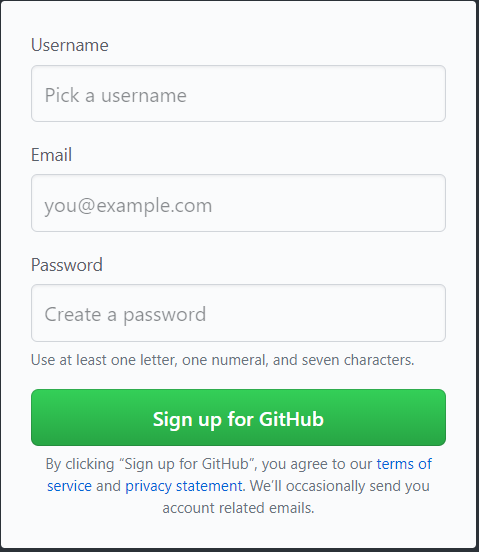
\includegraphics[scale=.5]{GithubSignup.png} 
\caption{The Sign Up textboxes on the main page of GitHub.}
\end{center}
\end{figure} 

Once these are filled in, select the green ``Sign up for Github'' to create the account. The next pages offers a choice between a free account or a paid one. The paid version allows for the creation of private repositories, while the free one only allows public repositories, but includes all other features of GitHub. It is worth noting that shortly after creation of an account, you will receive an email asking you to verify your email address. It is as simple as clicking the link in the email, taking you to your account page on GitHub.

\hypertarget{proj-section}{\subsection{Start a Project}}

\subsubsection{Creating a Project Board}
Next, we want to be able to create projects to work on. To do this from the main repository page click the 
\includegraphics[scale=.5]{ProjectsTab.png} tab near the top. In the upper right hand corner of this tab, there will a green button like so, 
\includegraphics[scale=.5]{CreateAProject.png}. The next page will prompt you to choose a name for the project, as well as giving the option for a brief description. The final option we need to choose before creating the project is the template style. The default no template option will allow you to create your own columns for this project. This basic kanban option will automatically include \textit{To Do}, \textit{In Progress}, and \textit{Done} columns which will house issues that match those descriptions. 

\begin{center}
\begin{figure}[h!]
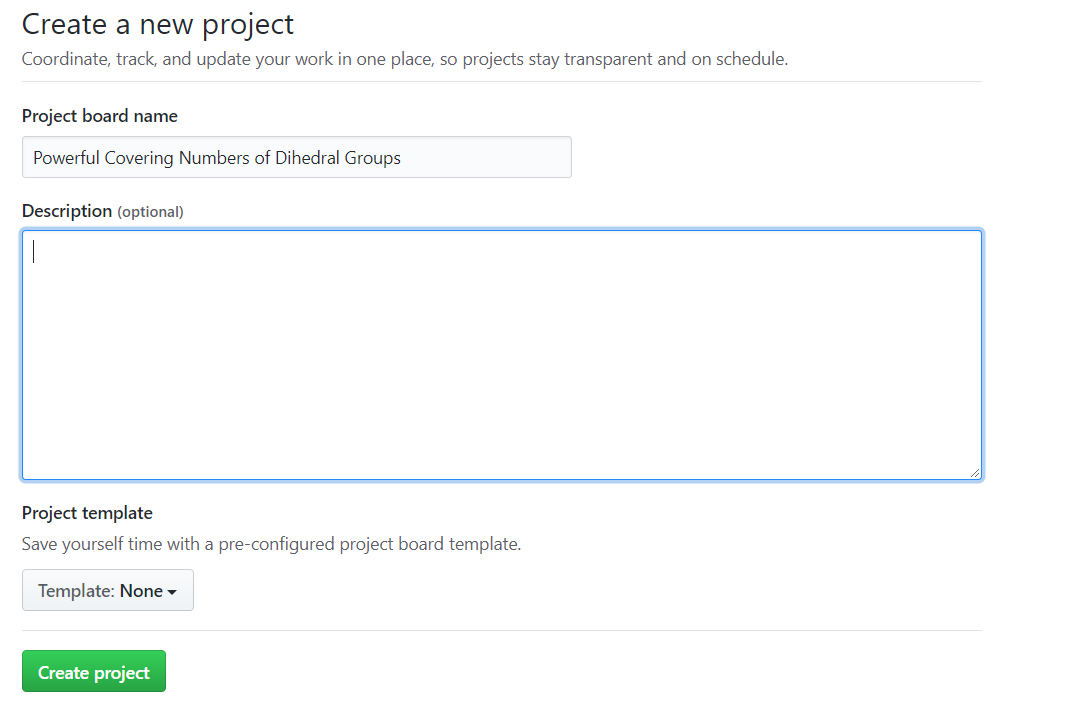
\includegraphics[scale=.6]{CreatingProject.png}
\caption{Creating a Project}
\end{figure}
\end{center} 
\subsubsection{Adding Columns to a Project Board}



\subsection{Add a File}

\subsubsection{From Your Computer} 

If you already have project files on your computer, you can upload them into the repository at any time by clicking the 
\includegraphics[width=0.5in]{UploadFilesbutton} from the repository screen. This will take you to a page where you can add files either by dragging into the window or by clicking to open a dialog box. When you first open a repository and do not have any files yet, you will be prompted to add files. 

\subsubsection{From Overleaf}

\subsection{Edit a File}

\section{Collaborators}

\subsection{Invite a Collaborator} 

\textbf{To invite someone to work on a repository with you},

\begin{enumerate}
\item Go to the repository.
\item Click the 
\includegraphics[width=0.75in]{SettingsButton} button.  
\item From the ``Settings'' page, click on the \includegrpahics[width=0.75in]{CollaboratorsButton} button on the left side of the page.
\item Type the information into the search window \begin{center} 
\includegraphics[width=0.8\textwdidth]{CollaboratorSearch}
\end{center}
and click ``Add a Collaborator''. 
\end{enumerate}

\subsubsection{Being Invited as a Collaborator}

If you know that you have been invited to collaborate on a project, you can accept the invitation to collaborate by going to the repository at the link \url{https://github.com/username/reponame/invitations}, where \texttt{username} and \texttt{reponame} are replaced in the obvious way. 

You will also receive an e-mail notifying you of the invitation to collaborate. You will \textbf{not} see anything in your GitHub notifications. 

\hypertarget{issues-section}{\subsection{Issues}}

Issues are a way for team members to communicate and keep track of changes to the project.  Here is GitHub's description of an issue:~\cite{github-issues} \\

\begin{quote}
Issues are used to track todos, bugs, feature requests, and more. As issues are created, they'll appear here in a searchable and filterable list. To get started, you should \underline{create an issue.}
\end{quote} 

\subsubsection{Creating An Issue}
We'll follow their advice, creating our first issue. The first issue we will create will be a ``\texttt{todo}'', telling us to create an issue. (Thus, this issue resolves itself.) We have two options: 

\begin{enumerate}

\item Under the 
\includegraphics{PlusMenu}
 in the upper left corner,we select the command ``New Issue''. \\

\begin{center}
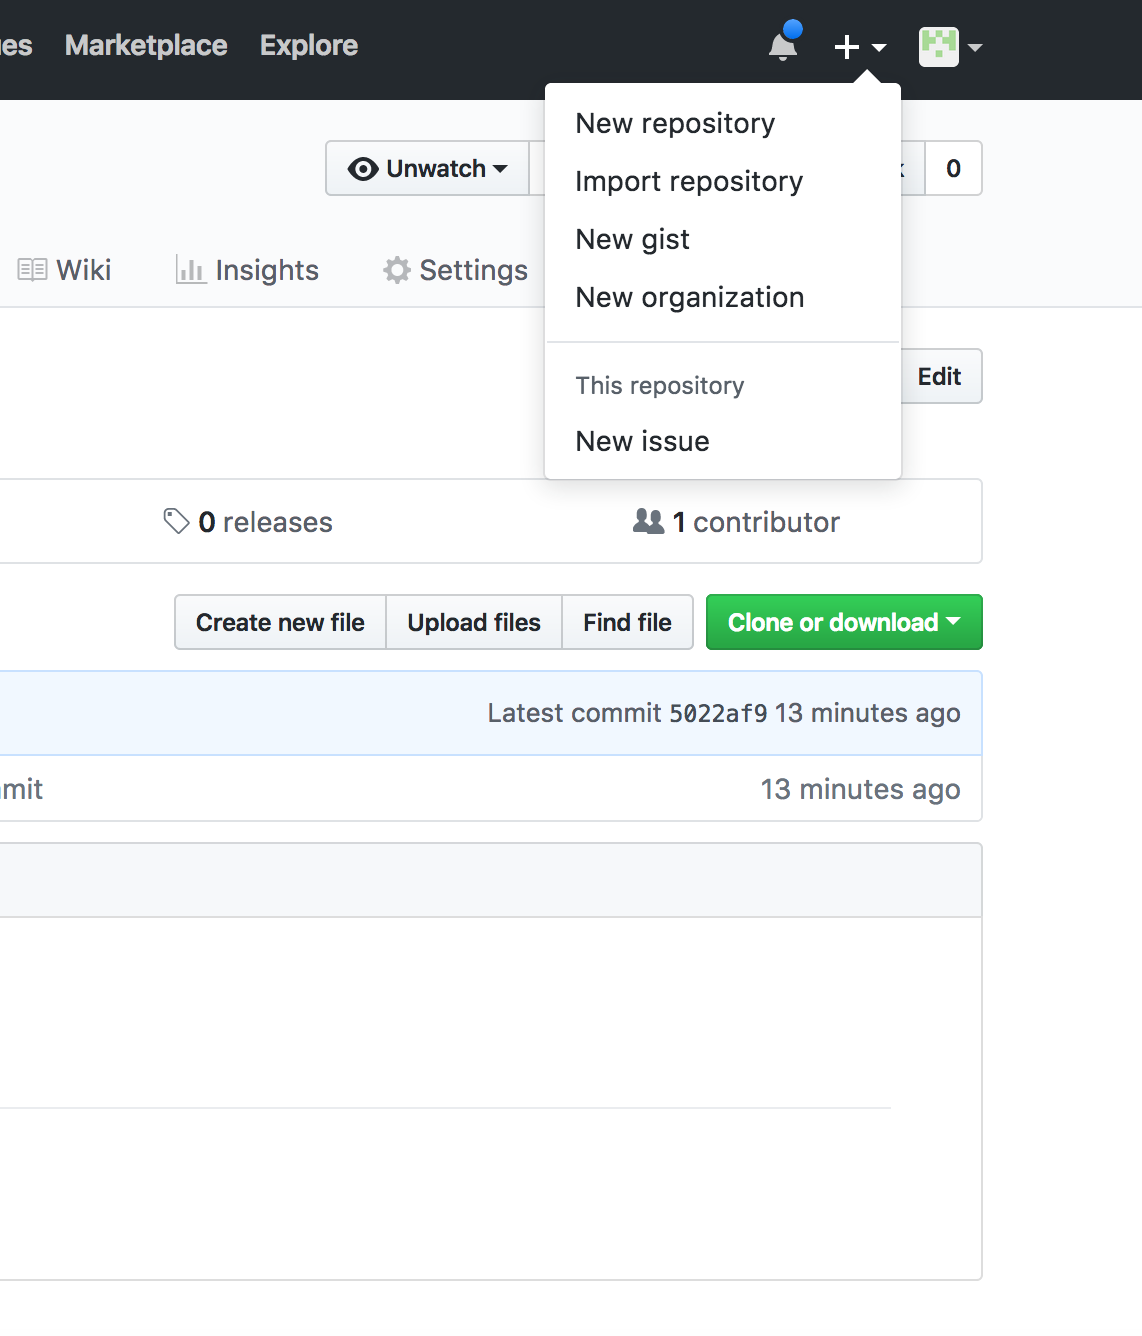
\includegraphics[width=0.5\textwidth]{NewIssueMenu}
\end{center}

\item We click on the 
\includegraphics[width=0.75in]{IssuesLink} tab, then click the 
\includegraphics[width=0.75in]{NewIssueButton} button. 

\end{enumerate} 

Either way brings up a ``New Issue'' screen with fields for Title and Description. We fill in this information, then click the 
\includegraphics[width=0.75in]{SubmitNewIssue} button. 

\begin{center}
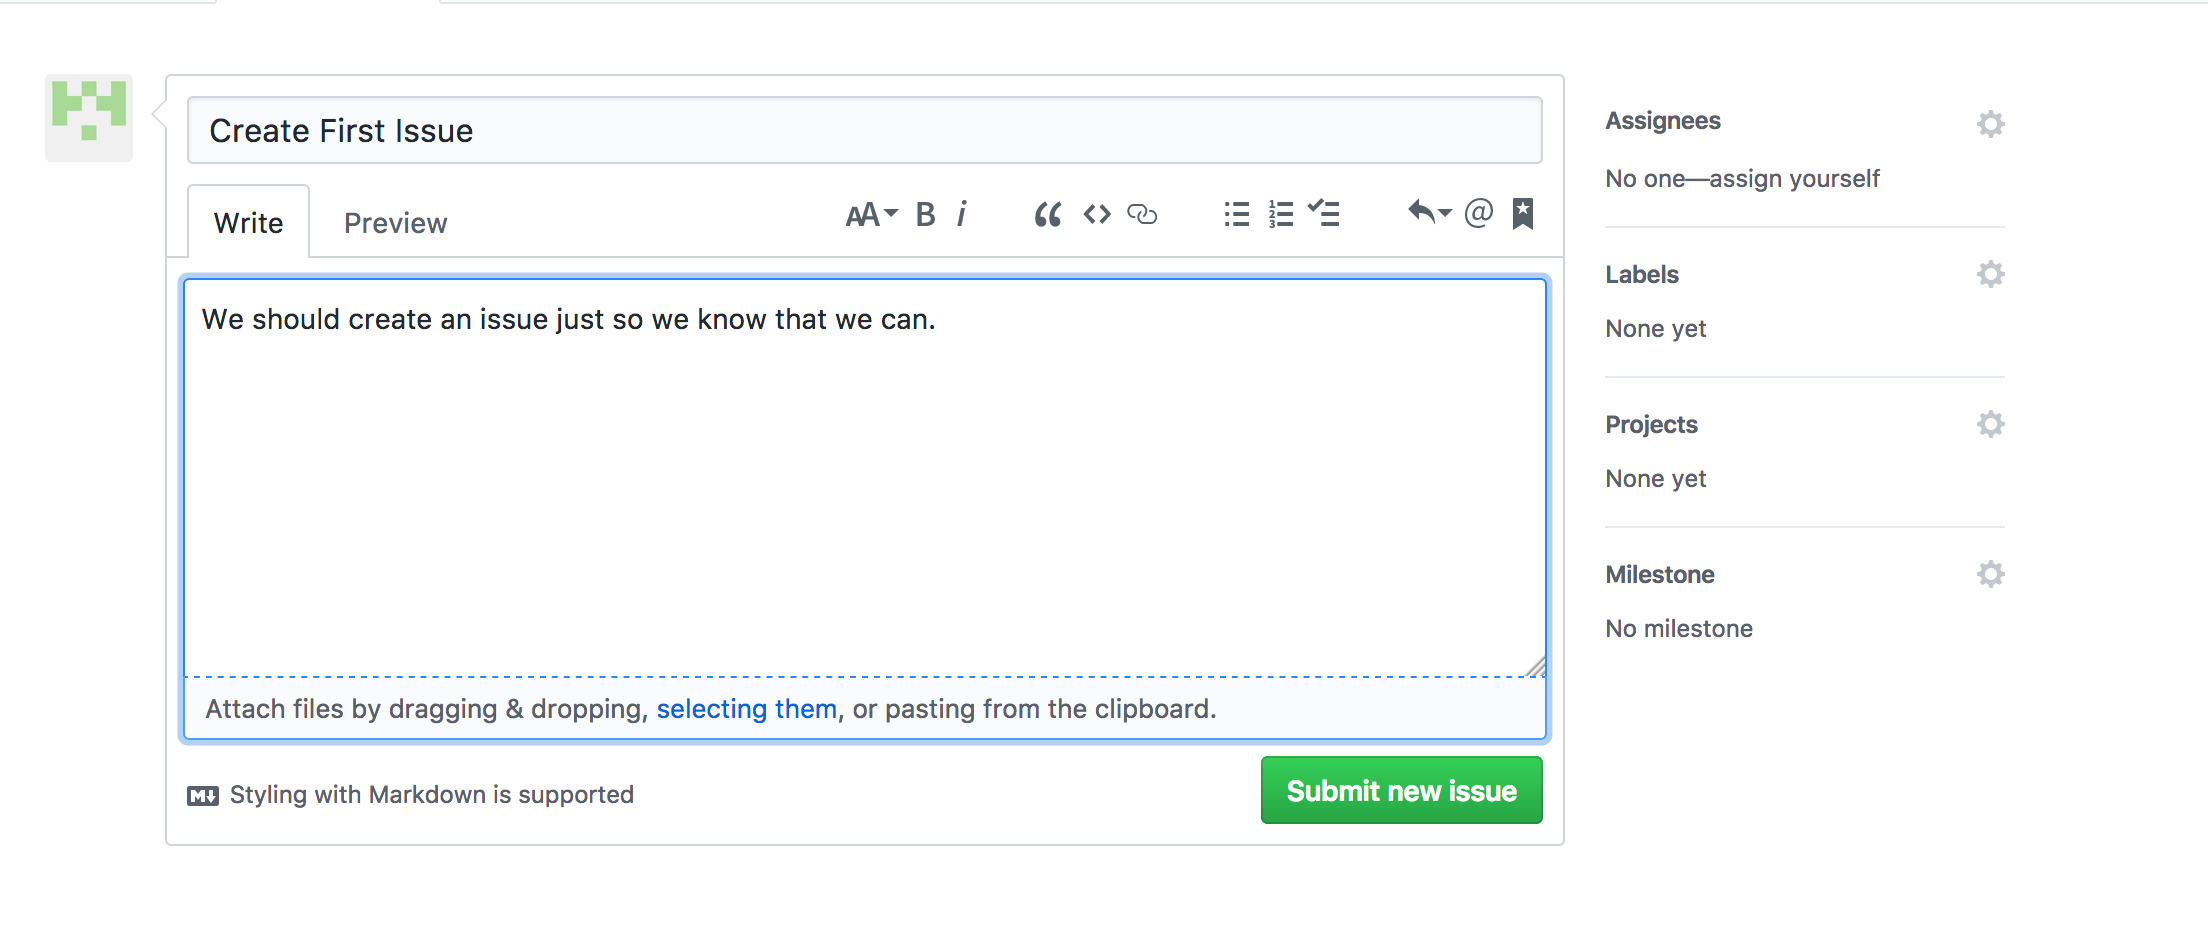
\includegraphics[width=\textwidth]{CreatingAnIssue}
\end{center}

\subsubsection{Checking For Issues}

If we log in to GitHub, we see that there is a new Issue by checking the ``Issues'' tab. We see 
\includegraphics[width=0.75in]{IssuesLink}, telling us there is one new issue. We click on the tab to see what the issue is.

\subsubsection{Closing An Issue} 

Once an issue is satisfactorily resolved, we want to close it. We can do this on the Issues screen by selecting the checkbox next to the issue, then going to the ``Mark as'' menu and selecting ``Closed''.

\begin{center}
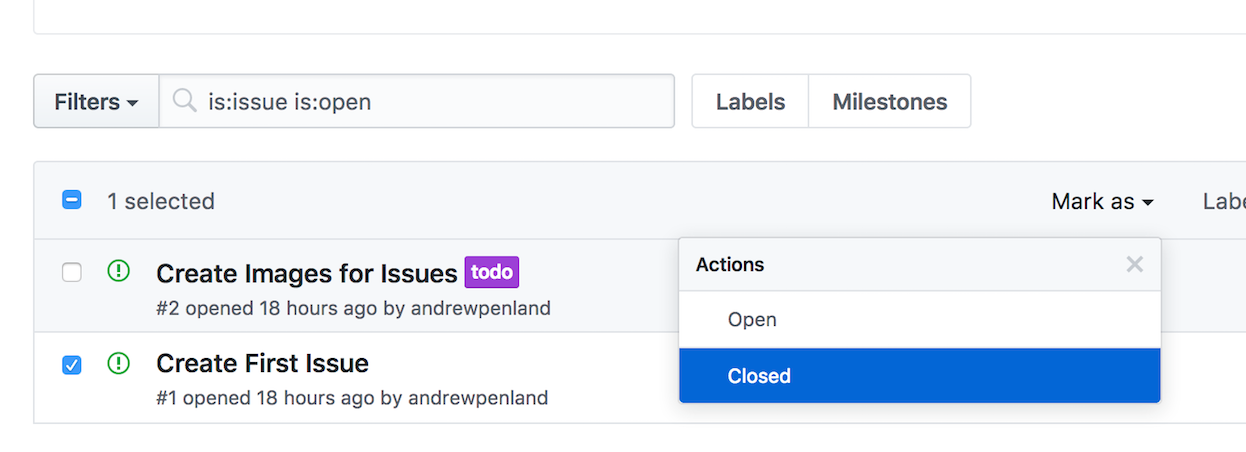
\includegraphics[width=0.9\textwidth]{MarkIssueClosed}
\end{center}

\subsubsection{Labeling Issues}

We can label issues so that we know what type they are. We can label an issue when we create it by using a dropdown menu called ``Labels''. GitHub has pre-existing labels for various categories. Simply type the name of the label you want to use or select it from the menu. 

\subsubsection{Creating Your Own Labels}

To create our own label, we begin by typing the name we want to use for the label. GitHub will automatically bring up a suggestion to create a label with this name.

Figure~\ref{fig:begin-typing-todo} and Figure~\ref{fig:todo-label-details} show how to create a ``todo'' label, which is a common issue that doesn't have a premade GitHub label. 


\begin{figure}\label{fig:begin-typing-todo}
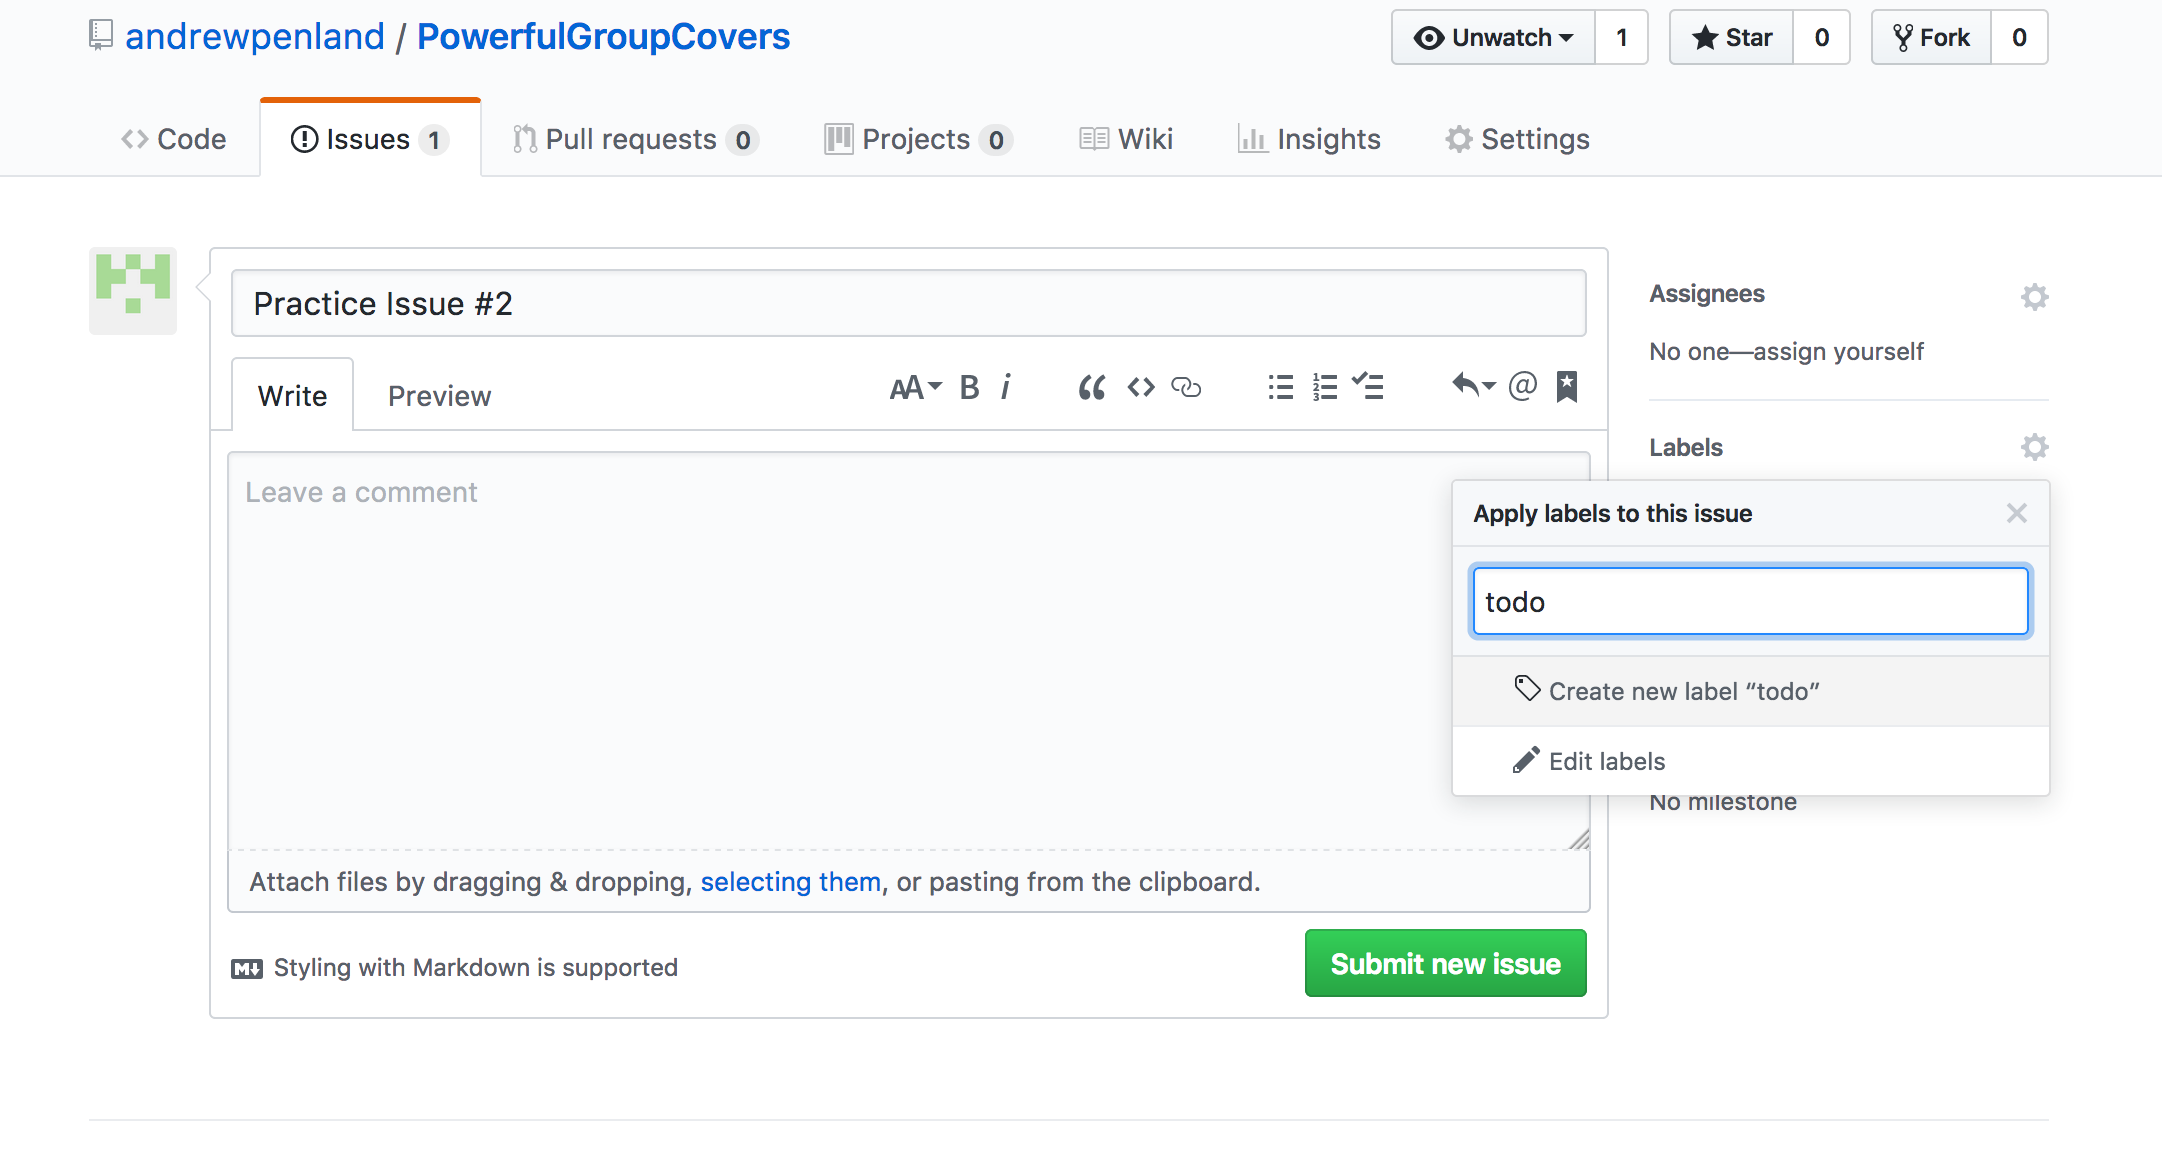
\includegraphics[width=0.9\textwidth]{CreatingLabels}
\caption{Labeling An Issue using The Menu}
\end{figure}

\begin{figure}\label{fig:todo-label-details}
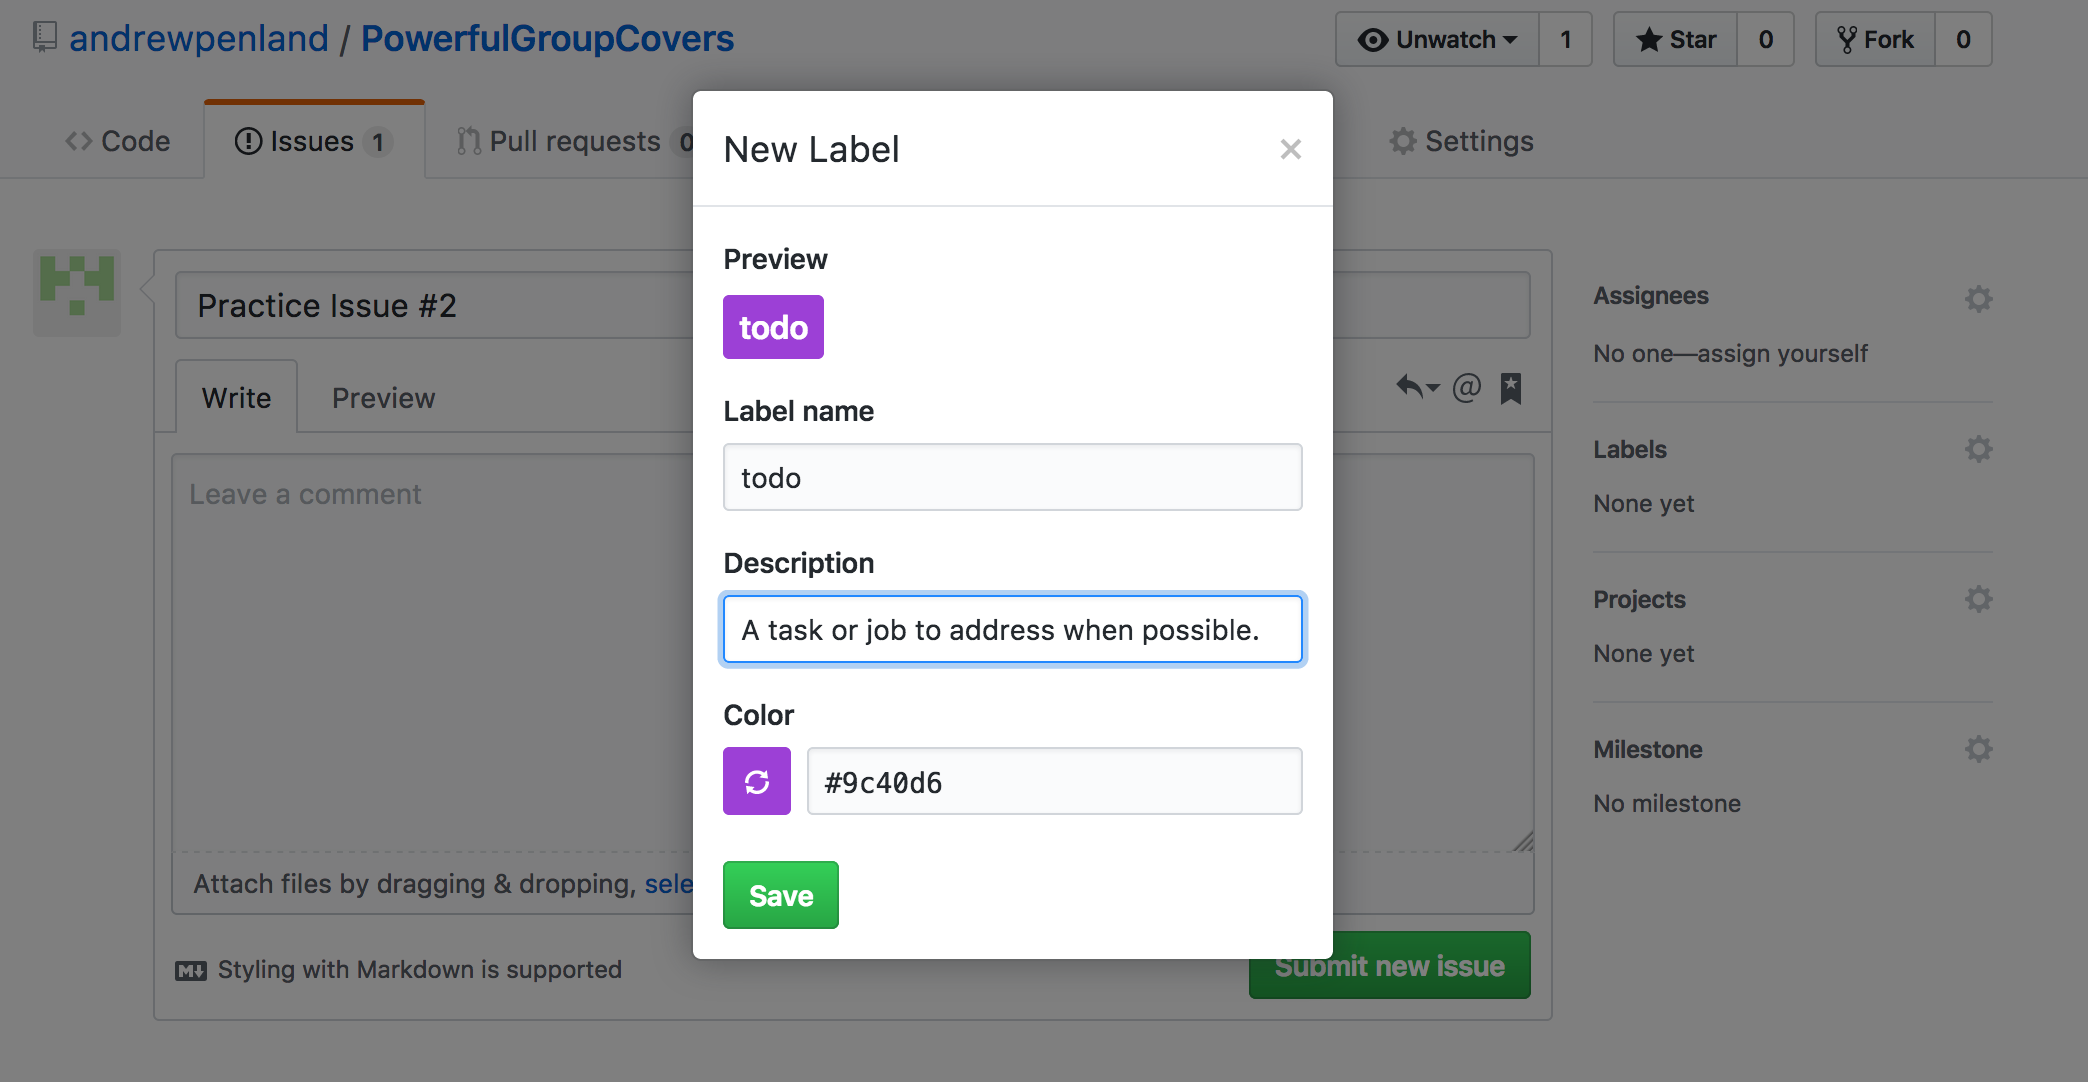
\includegraphics[width=0.9\textwidth]{NewLabelBox}
\caption{Creating A Custom Label}
\end{figure}


\subsubsection{Assigning Issues}

You can assign an issue to the attention of specific project members using the ``Assignments'' drop-down menu, which is to the right of the screen just above the ``Labels'' menu. 

\subsection{Pull Requests}

\subsection{Keeping Track of Changes}

\section{Conclusion}

\end{document}
